\input sys/inputs.tex

\usepackage{tikz}

\begin{document}

\bigheading{Poszterek}

% \info{task_name}{infile}{outfile}{points}{timelimit}{memlimit}
% leave this values, if you are not interested
\info{posters}{stdin}{stdout}{100}{1000 ms}{256 MB}

Mirek gyűjti kedvenc együttesének posztereit, amit a szobája falára tesz ki. Már sok posztere van, némelyiket már csak átfedéssel tudta kitenni. Szeretné tudni, hogy ha egy új posztert rakna ki egy adott helyre, akkor az mekkora területen takarná el a már ott lévő posztereket. 

\heading{Feladat}
Adottak a falon lévő poszterek koordinátái, valamint az új felrakandó poszterek tervezett koordinátái. Írj programot, amely minden új poszterre külön-külön kiszámítja, hogy mekkora területen takarná el a már ott lévő posztereket!

A már a falon lévő poszterek átfedhetik egymást, továbbá az átfedett területek csak egyszer számítanak. 

\heading{Bemenet}
A bemenet első sora a falon lévő poszterek $N$ egész számát tartalmazza ($1 \le N \le 100\,000$). A következő $N$ sor mindegyike egy, a már a falon lévő poszter koordinátáit tartalmazza. Az $N+2$. sorban a felrakandó új poszterek $M$ egész száma van ($1 \le M \le 100\,000$). Az ezt követő $M$ sor soronként egy új poszter koordinátáit tartalmazza.

Minden egyes poszter egy téglalap, amelynek oldalai párhuzamosak a koordináta-rendszer tengelyeivel. Minden poszter a bal alsó sarkának $x_1$, $y_1$ és jobb felső sarkának $x_2$, $y_2$ koordinátáival van megadva ebben a sorrendben ($0 \le x_1 < x_2 \le 10^9$, $0 \le y_1 < y_2 \le 10^9$).

\heading{Korlátok}
A tesztesetek $50\%$-ában a koordináták értékei legfeljebb $30\,000$.

\heading{Kimenet}
Minden egyes új poszter esetén a kimenetre egyetlen egész számot, az új poszter által eltakart terület nagyságát kell kiírni. A válaszokat az új poszterek bemenetbeli sorrendjében kell külön sorokba kiírni. 

\heading{Példa bemenet és kimenet}


\sampleIN
2
0 1 3 5
2 3 6 6
2
1 0 5 4
4 2 7 7
\sampleCOMMENT
Mirek falát az alábbi ábra szemlélteti.
A besatírozott téglalapok a már a falon lévő posztereket  jelölik, a szaggatott vonallal rajzolt téglalapok pedig az új felrakandó posztereket.
\begin{center}
	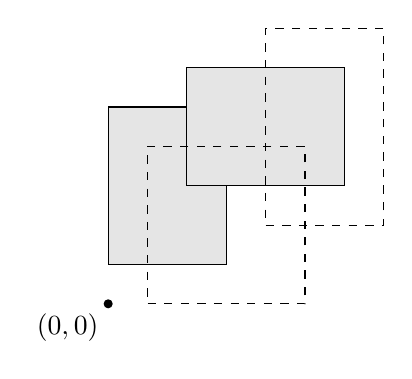
\begin{tikzpicture}[scale=0.5]
		\filldraw (0, 0) node[below left] {$(0, 0)$} circle(0.1);
		\filldraw[gray!20] (0, 1) -- (3, 1) -- (3, 5) -- (0, 5) -- cycle;
		\draw (0, 1) -- (3, 1) -- (3, 5) -- (0, 5) -- cycle;
		\filldraw[gray!20] (2, 3) -- (6, 3) -- (6, 6) -- (2, 6) -- cycle;
		\draw (2, 3) -- (6, 3) -- (6, 6) -- (2, 6) -- cycle;
		\draw[dashed] (1, 0) -- (5, 0) -- (5, 4) -- (1, 4) -- cycle;
		\draw[dashed] (4, 2) -- (7, 2) -- (7, 7) -- (4, 7) -- cycle;
	\end{tikzpicture}
\end{center}
\sampleOUT
8
6
\sampleCOMMENT
\sampleEND


\end{document}
